\documentclass[12pt]{report}
\usepackage[utf8]{inputenc}
\usepackage[utf8]{vietnam}
\usepackage{amsmath}
\usepackage{amsfonts}
\usepackage{amssymb}
\usepackage{graphicx}
\usepackage{caption}
\usepackage{booktabs}
\usepackage{hyperref}
\usepackage{tabu}
\usepackage{indentfirst}
\usepackage{svg}
\usepackage{array}
\setlength{\parindent}{2em}
\renewcommand{\baselinestretch}{1.5}
\usepackage{tikz}
\usetikzlibrary{calc}
\usetikzlibrary{decorations.pathmorphing}
\usepackage{subcaption}
\usepackage{verbatim} 
\usepackage{listings}
\usepackage{lmodern}  % for bold teletype font
\usepackage{xcolor}   % for \textcolor
\setcounter{secnumdepth}{3}
\definecolor{light-gray}{gray}{0.95}
\renewcommand{\baselinestretch}{1.5}
\hypersetup{
    colorlinks=true,
    linkcolor=blue,
    filecolor=magenta,      
    urlcolor=cyan,
}




%\renewcommand{\familydefault}{\sfdefault}
 
%\renewcommand\thesection{\Roman{section}}
%\renewcommand\thesubsection{\arabic{subsection}}


%
%\title{LaTex Thesis Template}	%% title
%\author{Trương Ngọc Anh}			%% author's name

%
\newcommand{\argmax}{\arg\!\max}

\begin{document}
\begin{titlepage}
\begin{tikzpicture}[overlay,remember picture]
    \draw [line width=0.5mm,decorate,decoration={
        %,segment length=<length>,amplitude=<length>
        }]
        ($ (current page.north west) + (3cm,-3cm) $)
        rectangle
        ($ (current page.south east) + (-3cm,3cm) $);
\end{tikzpicture}

\begin{center}
	\textbf{ĐẠI HỌC QUỐC GIA TP.HỒ CHÍ MINH}\\
	TRƯỜNG ĐẠI HỌC BÁCH KHOA\\
	KHOA KHOA HỌC VÀ KỸ THUẬT MÁY TÍNH\\
	---------------o0o--------------- \\
	\vspace{5mm}
	
\includegraphics[scale=0.2]{charts/logo.png}
\end{center}
\vspace{5mm}

\begin{center}
	\textbf{Luận văn tốt nghiệp}
\end{center}

\textbf{\Large Phát hiện kẹt xe từ camera hành trình}

\vspace{5mm}

\textbf{GVHD: } TS.Dương Ngọc Hiếu

\vspace{5mm}

\textbf{Nhóm sinh viên thực hiện:}\par
\begin{tabular}{ c c }
 Trương Ngọc Anh & 1410141 \\ 
 Lê Nguyễn Minh Trí & 1414207     
\end{tabular}

\thispagestyle{empty}
\end{titlepage}
%
%\maketitle
\tableofcontents

%

%
\listoffigures
\listoftables
\chapter*{Lời cảm ơn}
Trước khi vào phần giới thiệu nội dung đề tài luận văn, nhóm sinh viên tụi em xin gửi lời cảm ơn chân thành và sự tri ân sâu sắc đối với thầy \textbf{Dương Ngọc Hiếu} đã giúp đỡ, hướng dẫn tận tình cho tụi em về những khái niệm căn bản và phương hướng tiếp cận thông qua việc phân tích ảnh được dùng trên công nghệ Deep Learning, giúp tụi em chỉnh sửa những thiếu sót trong quá trình nghiên cứu và thực hiện đề tài này. Ngoài ra, tụi em cũng xin chân thành cảm ơn anh \textbf{Nguyễn Thanh Trông} đã hướng dẫn, giúp đỡ tụi em về việc ứng dụng \& kết hợp Deep Learning với Big Data, bổ sung những thiếu sót, sai sót của tụi em trong quá trình thực hiện đề tài. Đồng thời, do những kinh nghiệm thực tiễn và phương hướng tiếp cận về công nghệ Deep Learning \& Big Data còn nhiều hạn chế nên bài luận văn không thể tránh khỏi những thiếu sót, tụi em rất mong sẽ nhận được ý kiến đóng góp từ phía Thầy, Cô để tụi em học hỏi thêm được nhiều kinh nghiệm và sẽ hoàn thành tốt đề tài luận văn này hơn nữa !
\begin{flushright}
Tụi em xin chân thành cảm ơn ! 
\end{flushright}
%\mainmatter
%
\chapter*{Lời mở đầu}

\section*{Vấn đề}
	 Từ những năm gần đây, tình trạng ùn tắc giao thông ở Tp.Hồ Chí Minh đã không dừng lại ở diễn biến phức tạp mà lại còn gia tăng hơn trước. Cụ thể, trên các tuyến đường hiện nay, tình trạng kẹt xe không chỉ xảy ra ở giờ cao điểm mà còn ở các khung giờ khác. Nguyên nhân dẫn đến sự việc trên, một phần ảnh hưởng bởi điều kiện thời tiết, một phần do các công trình cải tạo hạ tầng, khi thi công lấn chiếm mặt đường. Nhưng phần lớn là do mật dộ xe cộ ngày một đông dần, dẫn đến việc ùn ứ, ùn tắt, di chuyển chậm,... Từ những nguyên nhân đó, nhóm sinh viên chúng em đã xây dựng mô hình hệ thống phát hiện kẹt xe từ camera hành trình (cụ thể là camera hành trình xe buýt), với mong muốn có thể góp phần giải quyết được một phần nhỏ tình trạng giao thông hiện nay ở Tp. Hồ Chí Minh nói riêng cũng như ở Việt Nam nói chung.\par
\section*{Động lực nghiên cứu và tính cấp thiết của đề tài}
	Trong bối cảnh mà các công nghệ xử lý trở phát triển mạnh như hiện nay. Chúng ta có thể áp dụng các công nghệ học máy và deep learning trong nhiều linh vực khác nhau từ y tế, nông nghiệp, kinh tế tài chính... Kèm theo đó là lượng dữ liệu tăng đột biến. Sẽ thật tốt nếu có một hệ thống vừa có thể lưu trữ dữ liệu lớn mà vừa có khả năng áp dụng công nghệ học máy, học sâu nói trên để hỗ trợ trong việc xử lý các vấn đề un tắt giao thông.\par 
	Khái niệm dữ liệu lớn, học máy, học sâu nhiều năm gần đây. Khi chính công ty lớn điển hình là Google, hay Tesla cũng đang phát triển tạo ra các hệ thống hỗ trợ giao thông thông minh. Các nước phát triển với các đặc tính dân số đông, mật độ giao thông phức tạp như Trung Quốc cũng đã ráo riết xây dựng các hệ thống camera giám sát kết hớp với học sâu để tiến hành nhận diện ảnh giao thông..v.v.\par 
	Đối với trong nước, hiện nay nhà nước cũng đã bắt đầu tiến hành đâu tư các hạng mục giao thông, thực hiện việc trang bị các camera giám sát tại một số tuyến đường trọng tâm nhằm để theo dõi tinh trạng giao thông. Nhưng để áp dụng linh vực học sâu hay thậm chí là xử lý ảnh vào để sử dụng thì vẫn còn khan hiếm.\par 
	Như vậy, môt hệ thống có thể lưu trữ kết hợp với lĩnh vưc học sâu là thật sự cần thiết. Không phải chỉ cần thiết cho lĩnh vực giao thông, đây có thể cân nhắc để trở thành một framework để ứng dụng để kết hợp các lĩnh vực khác nhau trong cuộc sống. Đây xứng đáng là một để nghiên cứu và phát triển. Với sự ra đời các mạng học sâu và các framework lưu trữ dữ liệu lớn như Apache Hadoop sẽ hỗ trợ cho việc nghiên cứu và phát triển hệ thống một cách dễ tiếp cận hơn. Chúng em đã nghiên cứu và lựa chọn ra mô hình mạng thích hợp cũng như xây dựng hệ thống mô phỏng lưu trữ dữ liệu lớn mà cho rằng có khả năng áp dụng vào thực tiễn.
	
\section*{Mục tiêu luận văn}		
Với các cơ sở thực tiễn trên, luận văn này đặt ra các mục tiêu như sau:
\begin{itemize}
	\item Lựa chọn, áp dụng mô hình mạng phân loại ảnh giao thông.
	\item Xây dựng hệ thống mô phỏng lưu trữ dữ liệu lớn.
	\item Kết hợp mạng học sâu với hệ thống lưu trữ dữ liệu lớn.
\end{itemize}

\section*{Giới hạn đề tài}
\begin{itemize}
	\item Hướng tới xây dựng mô hình hệ thống phân loại và lưu trữ dữ liệu lớn.
	\item Áp dụng các kiến trúc mạng mã nguôn mở.
	\item Do hướng tới xây dựng hệ thống và áp dụng các kết quả từ các công trình đã có nên luận văn sẽ không chú trọng vào việc cải thiện thuật toán hay đi sâu vào các kiến thức trong lĩnh vực xử lý ảnh.
\end{itemize}

\section*{Tính khả quan}
	Đề đánh giá về tính khả quan trong đề tài này, chúng ta cần phân tích một số đặc điểm. Thứ nhất là về tập ảnh giao thông, tập ảnh giao thông tốt hay không tuỳ thuộc vào nhiều yếu tố như nguồn gốc tập ảnh hay cơ cấu hạ tầng camera giao thông được đầu tư như thế nào. Đối với thành phố Hồ Chí Minh nói riêng, chúng ta vẫn còn đang xây dựng hệ thống cơ sở hạ tầng giám sát nên chưa thể dựa vào nguồn camera giám sát để lấy dữ liệu. Vì thế, chúng em sẽ sử dụng tập ảnh từ camera hành trình trên các xe buýt để thực hiện xây dựng mô hình. Khi đã có tập dữ liệu đủ tốt, chúng ta có thể sử dụng mô hình được xây dựng trên đề tài này và có thể được áp dụng vào hệ thống thực tiễn.

\section*{Cấu trúc luận văn}
\begin{itemize}
	\item \textbf{Chương 1: Tổng quan về hệ thống phân loại ảnh giao thống kết hợp với lưu trữ dữ liệu lớn.} Giới thiệu sơ lược về vấn đề đặt ra trong luận văn, các nghiên cứu đã có trên thế giới và hướng tập trung nghiên cứu.
	\item \textbf{Chương 2: Mạng neural và Mạng neural tích chập (Convolutional Neural Networks CNN.} Cơ sở lý thuyết về mạng học sâu.
	\item \textbf{Chương 3: Apache Hadoop.} Tổng quát framework lưu trữ dữ liệu lớn Apache Hadoop.
	\item \textbf{Chương 4: Phương pháp giải quyết.} Đề xuất giải pháp cho đề tài.
	\item \textbf{Chương 5: Hiện thực mô hình loại ảnh giao thông kết hợp Apache Hadoop. }Hiện thực giải pháp đã chọn cho hệ thống phân loại. Bao gồm nội dung về cài đặt va huấn luyện mạng học sâu đã chọn.
	\item \textbf{Chương 6: Kết quả huấn luyện và đánh giá.} Kết quả và các đánh giá vê kết quả đạt được.
	\item \textbf{Chương 7: Kết luận.}
\end{itemize}\newpage\cleardoublepage
\chapter{Mạng neural và Mạng neural tích chập (Convolutional Neural Networks CNN}

\section{Mạng neural (Neural Network)}

\subsection{Mạng neural ( Neural Network )}
	
	
	Theo khái niệm về sinh học, mạng neural là sự kết nối giữa các tế bào thần kinh neural lại với nhau. Trong lĩnh vực trí tuệ nhân tạo, mạng neural còn được gọi là Artificial Neural Network (ANN) - mạng neural nhân tạo, đây là mô hình xử lý dữ liệu, mô phỏng lại chức và cách hoạt động của hệ thống neural sinh học ở con người. Hình \ref{fig:neuron} minh họa cấu trúc của tế bào thần kinh neuron.
	
	\begin{figure}[h!]
		\centering
		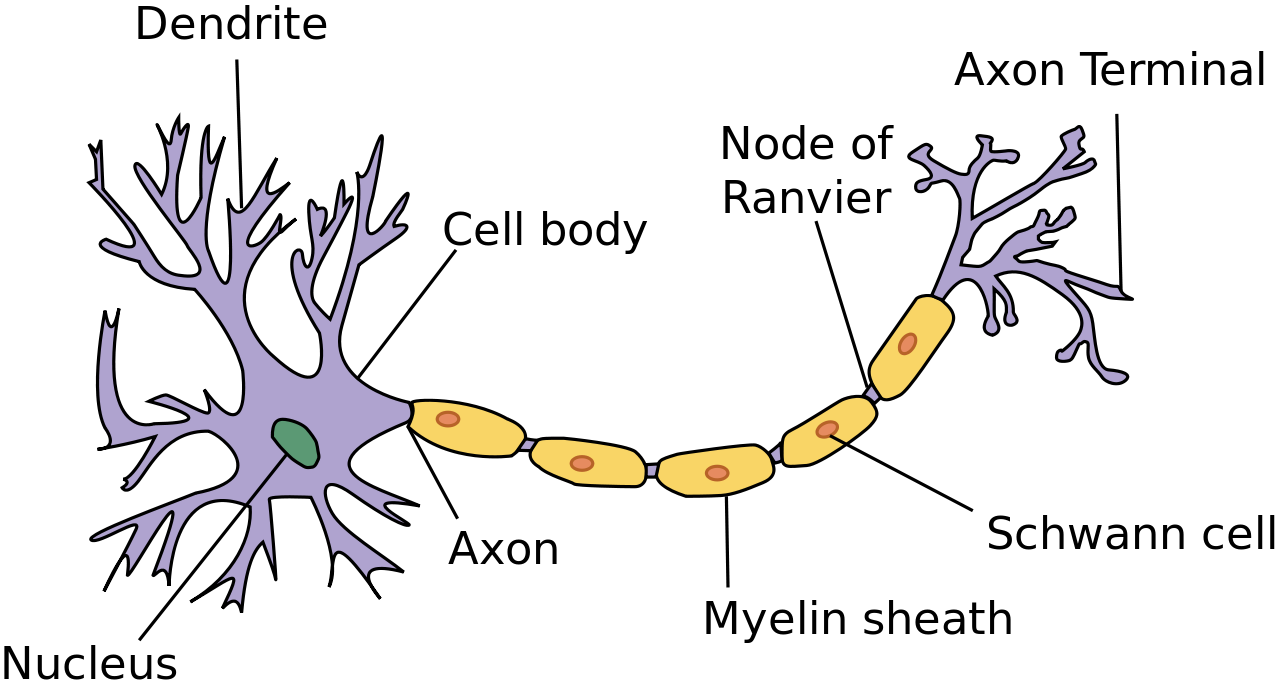
\includegraphics[scale=0.18]{charts/neuron.png}
		\caption{Tế bào thần kinh neuron sinh học}
		\label{fig:neuron}
	\end{figure}
	
	Mạng neural có gồm nhiều đơn vị kết nối, làm việc như một thể thống nhất thông qua việc trao đổi thông tin nhờ các liên kết.
	
	\subsection{Cấu trúc mạng neural}
	Như đã trình bày, các neuron trong một mạng làm việc như một thể thống nhất bằng việc trao đổi thông tin. Thực tế, đây là quá trình điều chỉnh các trọng số được truyền từ input ban đầu kết hợp với các hàm tính toán để có được các thông số trọng số phù hợp nhất. Quá trình này còn được gọi là quá trình học hay huấn luyện. Hình \ref{fig:NN} mô tả cấu trúc đơn giản nhất của một mạng neuron.
	\begin{figure}[h!]
		\centering
		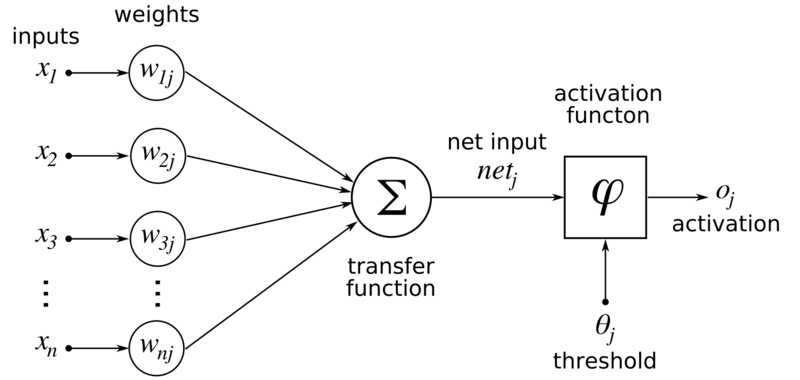
\includegraphics[scale=0.4]{charts/NN.png}
		\caption{Cấu trúc cơ bản mạng neuron}
		\label{fig:NN}
	\end{figure}
	
	\textbf{Cấu trúc mạng neuron\i}
	
	\begin{itemize}
		\item \textbf{Tập các node:} bao gồm nhiều node, mỗi node là đơn vị nhỏ nhất giữ chức năng xử lý thông tin của mạng.
		\item \textbf{Các tầng:} Các node trên được xếp thành các tầng, các node chung một tầng không thể kết nối nhau. Trong đó tầng input và tầng output là 2 tầng thiết yếu. Tùy vào một số mạng cụ thể có thể có thêm một hay nhiêu tầng nằm ở giữa được gọi là tầng ẩn (hidden layer).
		\begin{itemize}
			\item \textbf{\textit{Tầng input - input layer: }}các nối ở tầng này nhận dữ liệu đầu vào và truyền tới các node ở các tầng kế tiếp, trong một số trường hợp còn có chức năng xử lý thông tin.
			\item \textbf{\textit{Tầng ẩn - hidden layer: }}một số mạng có thể có thêm tầng ẩn, số lượng tầng ẩn trong một mạng có thể nhiều hơn 1. Có chức năng nhận các giá trị từ từng input hoặc tầng ẩn trước nó, tính toán các giá trị và gửi đến các node ở các tầng ẩn hoặc tầng ouput tiếp theo đó tùy theo từng mạng cụ thể.
			\item \textbf{\textit{Tâng output - output layer: }}nhận giá trị từ tầng trước đó (tầng ẩn hoặc tầng input) để tính toán các giá trị ngõ ra.
		\end{itemize}
		\item \textbf{Các liên kết:} mỗi node trong một tầng truyền thông tin qua các node ở các tầng khác thông qua các liên kết. Các giá trị mà các liên kết này được gán sẽ được gọi là trọng số liên kết (weight). Giá trị trọng số được kết nối vào neuron j với neoron k là \(w_{kj}\).
		\item \textbf{Hàm truyền - transfer function: }dùng để tính tổng các tích input với trọng số liên kết của nó. \[ \sum input_j*w_{ij}\]
		
		\item \textbf{Activation function: }dùng để tính toán giá trị input sang giá trị ouput. Tùy vào mục địch và cụ thể từng loại mạng mà có nhiều loại activation function khác nhau.\\
		Trong các bài toán khác nhau, người có những loại hàm activation như sau.
		
		\begin{itemize}
			\item \textbf{\textit{Step function: }} 
			\[ 
			\left \{
  			\begin{tabular}{cc}
  				0 & x < 0\\
  				1 &  x > 0 
  			\end{tabular}
		\right.
		\]
		\pagebreak
		\begin{figure}[h!]
			\centering
			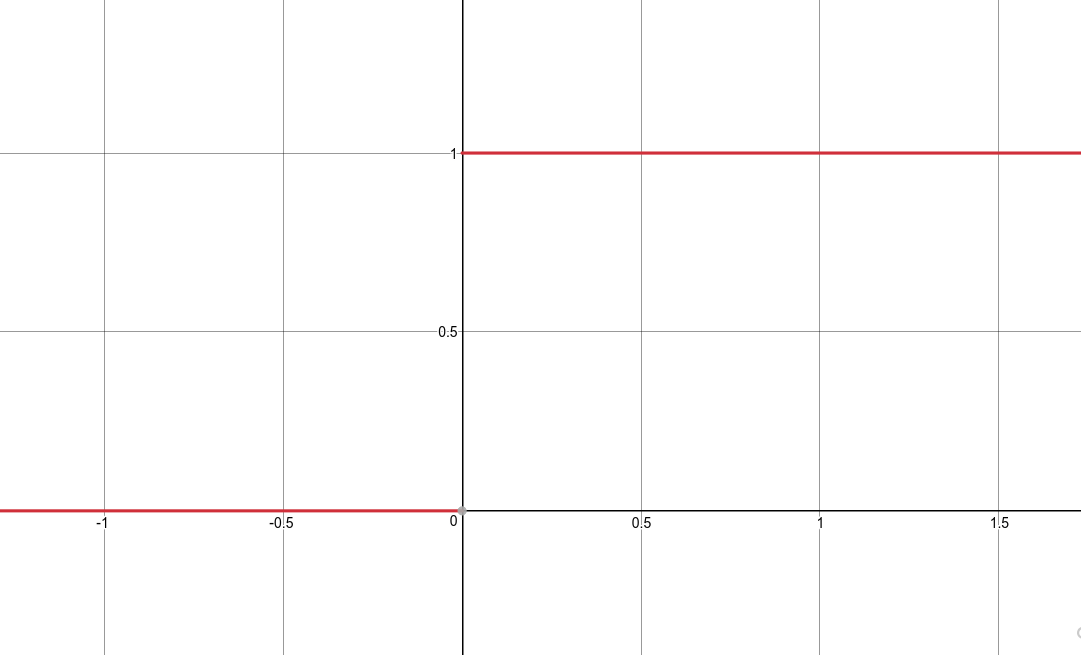
\includegraphics[scale=0.2]{charts/step_fun.png}
			\caption{Đồ thị hàm step}
			\label{fig:plot_step}
		\end{figure}
		
			\item \textbf{\textit{sigmoid function: }}
			\[A(x) =  \frac{1}{1 + e^{-x}}	\]
			\begin{figure}[h!]
				\centering
				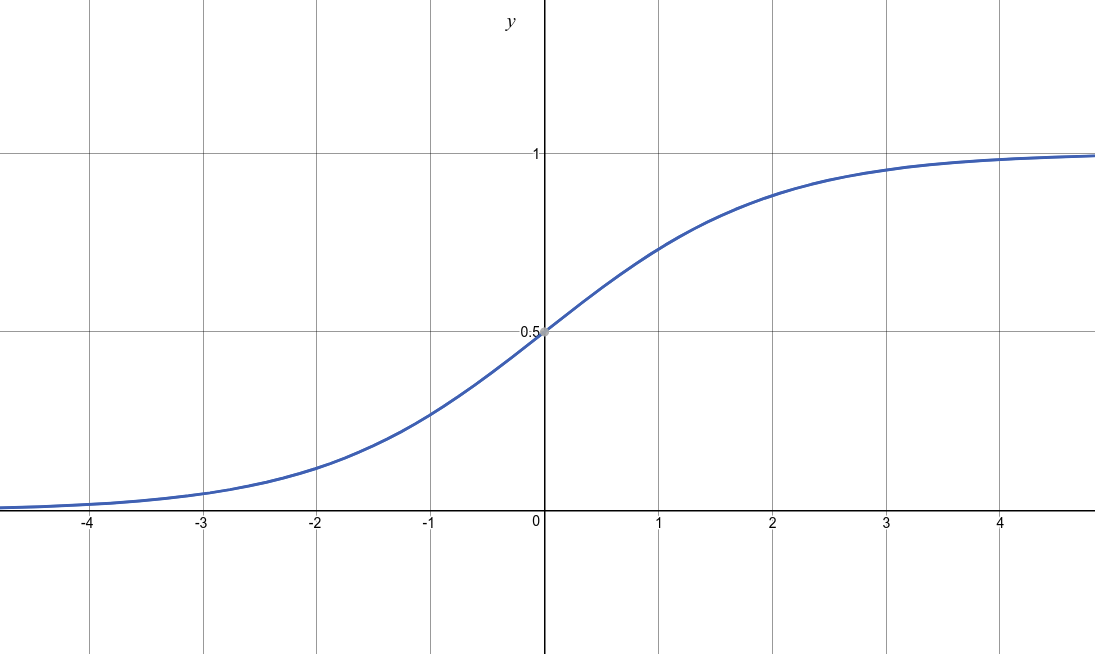
\includegraphics[scale=0.2]{charts/sigmoid_fun.png}
				\caption{Đồ thị hàm sigmoid}
				\label{fig:plot_sigmoid}
			\end{figure}
			
			\item \textbf{\textit{Tanh function:}}
			\[Tanh(x) = \frac{2}{1 + e^{-2x}} - 1 \]
			\begin{figure}[h!]
				\centering
				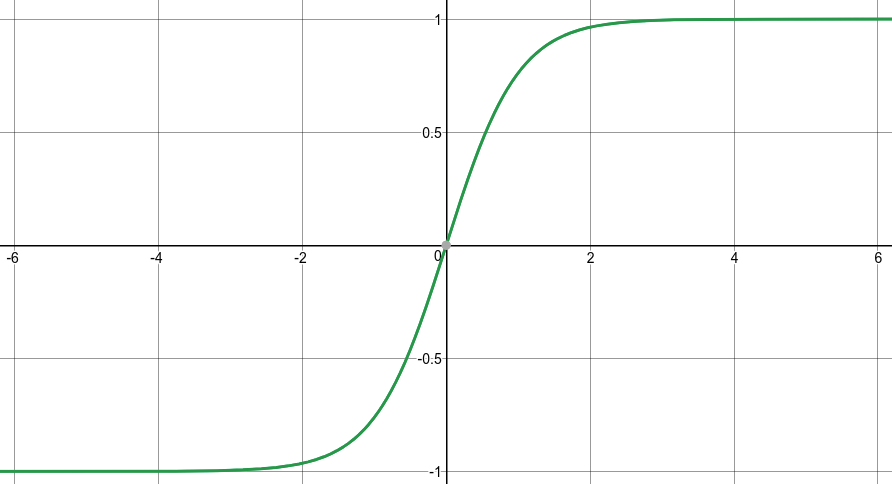
\includegraphics[scale=0.2]{charts/tanh_fun.png}
				\caption{Đồ thị hàm Tanh}
				\label{fig:plot_tanh}			
			\end{figure}
			
		\end{itemize}
		
	\end{itemize}
	
	\subsection{Mô hình Feedforward Neural Network}
	
		Thời điểm hiện nay, chúng ta có rất nhiều loại mô hình mạng neuron do sự khác nhau về sự kết hợp cũng như về mặt kiến trúc và thuật toán mà mạng đó áp dụng. Trong phần này, chúng ta sẽ tìm hiểu về mô hình mạng Feedforward Neural Network (FFNN), đây là kiến trúc mạng neuron được sử dụng phổ biến trong các bài toán dự báo. Mô hình gồm hai thành phần chính đó là kiến trúc feedforward - mạng truyền thẳng và giải thuật Backpropogation được áp dụng trong mạng.
		\subsubsection{Kiến trúc Feedforward}
			Đối với mạng feedfroward, cấu trúc gồm một tầng input, một tầng output và có thể có nhiều hơn một tầng ẩn nằm giữa hai tầng input và output. \\
			\begin{figure}[h!]
				\centering
				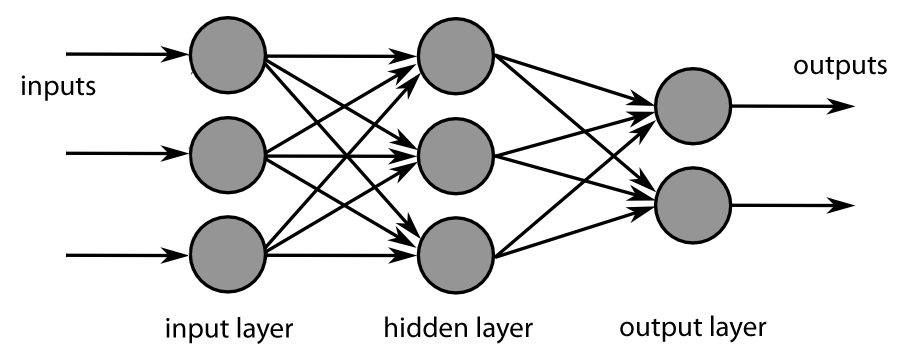
\includegraphics[scale=0.3]{charts/ffnn.png}
				\caption{Ví dụ kiến trúc mạng feeddorward}
				\label{fig:ffnn}			
			\end{figure}\\
			Như hình \ref{fig:ffnn}, một mạng Feedorward, trong tầng input và ouput thì số lượng neuron tại mỗi hai tầng nãy sẽ là cố định tùy theo đặc tính của dữ liệu. Đối với tầng ẩn, số lượng tầng ẩn cũng như số lượng neuron trong mỗi tầng tùy thuộc vào cá nhân thiết kế.
			
		\subsubsection{Giải thuật Backpropogation}
		Ở nội dung này, chúng ta sẽ không đi sâu vào kỹ thuật xử lý các phép tính\cite{dl} đạo hàm mà chỉ trình bày giải thuật lan truyền ngược một cách đơn giản nhất.\par
		Các ký hiệu và hàm được dùng trong trình bày giải thuật:
		\begin{itemize}
			\item \(W_{ij}\): là trọng số nối node thứ i tới node j ở layer kế tiếp.
			\item \(I_{j}\): là đầu vào tại node thứ j.
			\item \(O_{j}\): là kết quả xuất tại node thứ j.
			\item \(\theta_{j}\): bias tại node j.
			\item \(l\): tốc độ học của mạng (learning rate).
			\item \(Err_{j}\): giá trị lỗi tại node thứ j.
			\item Activation function được dùng trong nội dung này là hàm Sigmoid như mục trên
		\end{itemize}
		
		\begin{figure}[h!]
			\centering
			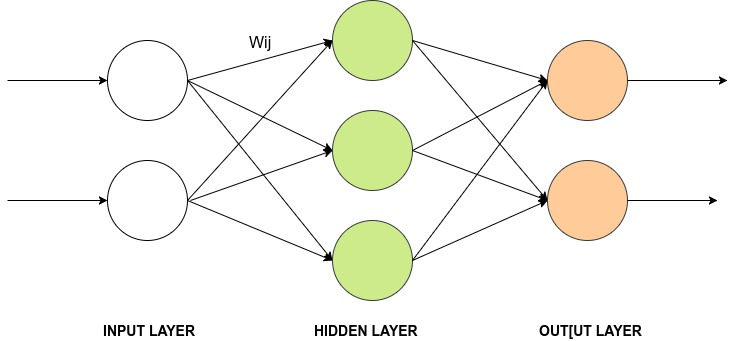
\includegraphics[scale=0.5]{charts/back.jpg}
			\caption{MLP}
			\label{fig:back}
		\end{figure}
		\pagebreak
		Nội dung thuật toán.\par
		\textbf{Input:}
		\begin{itemize}
			\item Mạng feed forward với n input, m node ở tầng ẩn, và p output.
			\item Hệ số học hay tốc độ học \(l\).
			\item Tập dữ hiệu huấn luyện \(D\).
			\item Sai số học \(\epsilon\).
		\end{itemize}
		\textbf{Output:} Vector các trọng số mới sau khi huấn luyện.
		
		\textbf{Nội dung thuật toán:}
		
		\begin{itemize}
			\item \textbf{Bước 1:} Khởi tạo ngẫu nhiên các giá trị trọng số  \(W_{ij}\).
			\item \textbf{Bước 2:} Tính toán các giá trị đầu vào \(I_{j}\) và đầu ra \(O_{j}\).
			\begin{itemize}
				\item Tại node i ở tầng input:
				\[I_{i} = x_{i}, O{i} = I_{i}\]
				\item Tại node j ở tầng khác:
				\[ I_{j} = \sum_{i} W_{ij}O_{i} + \theta_{j} \]
				\[O_{j} = \frac{1}{1 + e^{-I_{j}}}\]
			\end{itemize}
			\item \textbf{Bước 3:} Tính toán lỗi trung bình và đánh giá.
				\begin{itemize}
					\item Tại node thuộc tầng output:
					\[Err_{j} = O_{j}(1-O_{j})(T_{j} - O_{j})\]
					\item Tại node thuộc tầng ẩn:
					\[Err_{j} = O_{j}(1-O_{j})\sum_{k}Err_{k}W_{jk}\]
					Với \(Err_{k}, W_{jk}\) là giá trị lỗi tại node k ở tầng tiếp theo và giá trị trọng số của node j đến k.\\
					Thuật toán sẽ dừng lại khi \(Err_{k} \leq \epsilon\)
					
				\end{itemize}
			\item \textbf{Bước 4:} Cập nhật các trọng số và độ lệch
			\[W_{ij} = W_{ij} + (l)Err_{j}O_{i}\]
			\[\theta_{j} = \theta_{j} + (l)Err_{j}\]
			
			Thuật toán sẽ tiếp tục lặp lại bước 2 cho đến khi thỏa điều kiện dừng và cho ra các tập trọng số và độ lệch tốt nhất.
		\end{itemize}
		
		
		
		
			
			

\section{Mạng neural tích chập (Convolutional neural network)}

\subsection{Giới thiệu mạng neural tích chập}
	Trong vài năm trở lại đây, chúng ta thấy được sự nở rộ của các hệ thống thông minh từ các công ty công nghệ lớn trên thế giới. Các chức năng nhận dạng, phân loại hay dự đoán được áp dụng rộng rãi vào các lĩnh vực thương mại, vận tải..v..v.\par
	Mô hình Deep learning được sử dụng phổ biến và phát triển giúp các hệ thống thông minh có độ chính xác cao ngày nay chính là Convolutional Neural Networks(CNN) - mạng neuron tích chập. Trong các nội dung tới, chúng ta sẽ tìm hiểu các khái niệm, kiến trúc, cũng như ứng dụng của CNN trong lĩnh vực phân loại ảnh.

\subsection{Mô hình mạng neural tích chập}
	\subsubsection{Input và output}
		Phân loại ảnh là công đoạn chuyển hóa từ một đầu là một hình ảnh và kết quả là một nhãn ứng với hình ảnh đó hoặc là các xác suất mà hệ thống dự đoán dựa trên đặc điểm của ảnh. Với con người, công việc nhận diện này được hình thành từ khi mới sinh ra, chúng ta có thể đưa ra kết quả của một hình ảnh bất kỳ mà không chút khó khăn. Nhưng máy tính thì không đơn giản như vậy, đầu vào và kết quả phải được đưa về dạng kỹ thuật số mà máy có thể hiểu được.\par
		Khi một máy tính nhận vào một ảnh, nó sẽ thấy một mảng các giá trị pixel tùy thuộc vào kích thước và độ phân giải của ảnh\cite{overview}. Ví dụ, một ảnh màu có kích thước 224 x 224 pixel thì máy tính sẽ thấy hình ảnh này dưới dạng một mảng có kích thước 224 x 224 x 3, giá trị 3 do thuộc tính ảnh màu(RGB) mà có được, giá trị này sẽ là 1 nếu đây là ảnh trắng đen.\par
		Đối với ouput, đây là một mảng các giá trị xác suất, mảng giá trị này cũng tùy thuộc vào số lượng nhãn(lớp) cần dự đoán. Ví dụ, (0.90 cho xe ô tô, 0.1 cho xe tải).
	\subsubsection{Convolutional layer}
		Tầng đầu tiên của một mạng CNN luôn luôn là tầng tích chập (convolutional layer)\cite{conv}. Như đã biết đầu vào (input) là một mảng các giá trị pixel. Trong trường hợp cụ thể để dễ hình dung ta chọn input là mảng các giá trị pixel có kích thước 32 x 32 x 3 với 32 x 32 là chiều dài và chiều rộng của tấm hình và 3 là giá trị RGB khi là ảnh màu. Đối với input trên có nghĩa là sẽ có một ma trận có kích thước 32 x 32 pixel mỗi pixel sẽ chứa 3 giá trị mà mỗi giá trị đó lần lượt biểu diễn cho giá trị của 3 màu sắc trên máy tính là đỏ(RED), lục(GREEN) và làm(BLUE). \par
		Tạm thời bỏ qua giá trị RGB để đi vào cách hoạt động của tầng tích chập này. Cách đơn giản để giải thích cách hoạt động của tầng tích chập là tưởng tượng sẽ có một khuôn sẽ trượt từ phía trên bên trái cho đến hết tấm ảnh\cite{arch}. Với kích thước ảnh là 32 x 32 như trên, chọn kích thước ô trượt ví dụ là 5 x 5. Ô trượt có kích thước 5 x 5 sẽ trượt lần lượt qua cả input ảnh, ô trượt này được gọi là kernel hay filter(bộ lọc). Bộ lọc là một mảng các giá trị trọng số. Một điểm ghi chú là chiều sâu của bộ lọc sẽ bằng với chiều sâu của ảnh, với input 32 x 32 x 3 thì bộ lọc cũng sẽ có 5 x 5 x 3. Hình \ref{fig:conv_layer1} và \ref{fig:conv_layer2} minh họa cách kernel trượt trên input.
		%\pagebreak
		\begin{figure}[h!]
			\centering
			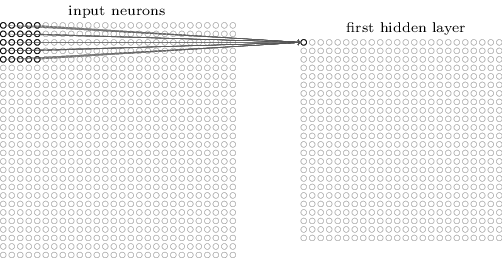
\includegraphics[scale=0.8]{charts/conv_layer1.png}
			\caption{Convolutional layer}
			\label{fig:conv_layer1}
		\end{figure}
		
		\begin{figure}[h!]
			\centering
			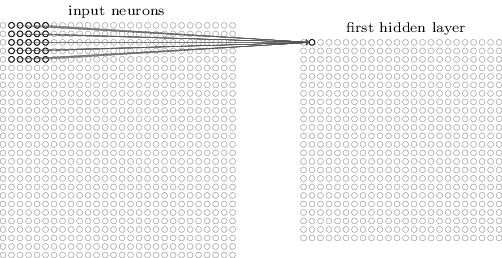
\includegraphics[scale=0.8]{charts/conv_layer2.png}
			\caption{Convolutional layer}
			\label{fig:conv_layer2}
		\end{figure}
		
		Bây giờ ta sẽ đi vào việc mà tầng tích chập thực sự làm với những phép tính. Như đã trình bày rằng mỗi bộ lọc sẽ là một mảng các giá trị pixel, công dụng của mảng giá trị này nhằm mục đích phát hiện các đặc tính của mỗi vùng input mà filter trượt qua. Các đặc tính ở đây có thể là đường thẳng, đường cong, màu đơn giản. Ví dụ ta có một filter có kích thước là 7 x 7 x 3 dùng để phát hiện một dạng đường cong như hình \ref{fig:filter}.
		
		\begin{figure}[h!]
			\centering
			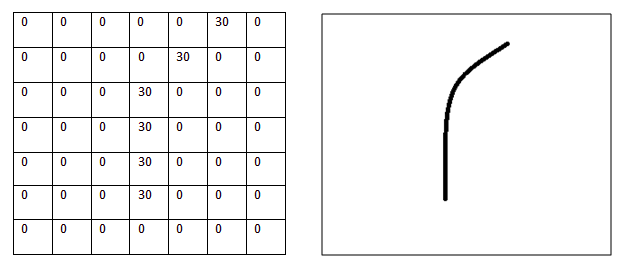
\includegraphics[scale=0.5]{charts/filter.png}
			\caption{Mảng các giá trị của bộ lọc}
			\label{fig:filter}
		\end{figure}
		
		Khi bộ lọc trên trượt đến vùng được đánh dấu vàng có dạng đường cong giống với bộ lọc như hình \ref{fig:mouse}. Lúc đó phép toán   tích châpj sẽ được thực hiện như hình \ref{fig:conv_1} với ma trận bên trái chính là giá trị pixel của vùng được đánh dấu trên ảnh mà bộ lọc trượt tới, ma trận bên phải chính là bộ lọc được sử dụng hiện tại.
		
		\begin{figure}[h!]
			\centering
			
\includegraphics[scale=0.5]{charts/mouse.png}
			\caption{ảnh đầu vào}
			\label{fig:mouse}
		\end{figure}
		\pagebreak
		
		\begin{figure}[h!]
			\centering
			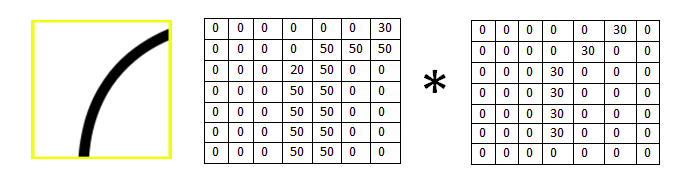
\includegraphics[scale=0.5]{charts/conv_1.png}
			\caption{phép toán tích chập}
			\label{fig:conv_1}
		\end{figure}
		
		Kết quả của phép tính trên sẽ có kết quả như sau:
		\[(50*30)+(50*30)+(50*30)+(20*30)+(50*30) = 6600 \]\\
	
		Đây là một con số rất lớn, thông thường nếu bộ lọc trượt tới một vùng mà vùng đó có hình dạng tương tự như bộ lọc thì kết quả khi thực hiện phép tính là một con số rất lớn. Ngược lại, kết quả sẽ ra rất nhỏ hoặc bằng 0. Ví dụ là hình ảnh \ref{fig:conv_2} kết quả sẽ là 0 khi thực hiện phép tính
		\begin{figure}[h!]
			\centering
			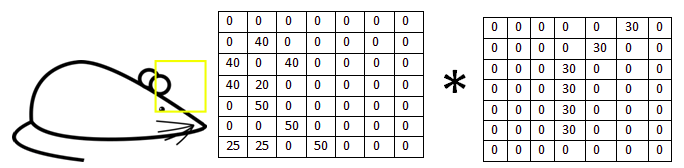
\includegraphics[scale=0.5]{charts/conv_2.png}
			\caption{phép toán tích chập}
			\label{fig:conv_2}
		\end{figure}
		
		Trên đây là mô tả đơn giản về tầng tích chập, trên thực tế, chúng ta có thể có nhiều bộ lọc để phát hiện các khuôn mẫu, hình dạng khác nhau trong ảnh đầu vào. Kết quả xuất của tầng tích chập thứ nhất còn được gọi là bản đồ đặc tính (feature map) và có thể có nhiều feature map cho một input sau khi hoàn thành tầng tích chập. Như \ref{fig:feature_map} biểu diễn một input kích thước như hình sau khi qua tầng tích chập và sử dụng tập các bộ lọc 5 x 5 cho ra tập 3 feature map mà mỗi cái nhận diện được một khuôn dạng khác nhau xuất hiện trong input.
		%\pagebreak
		\begin{figure}[h!]
			\centering
			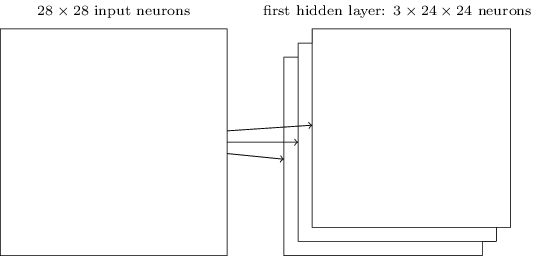
\includegraphics[scale=0.5]{charts/feature_map.png}
			\caption{kết quả tầng tích chập}
			\label{fig:feature_map}
		\end{figure}
	
	\subsubsection{Pooling Layer}		
		Sau khi qua một hoặc vài tầng tích chập, CNN sẽ chứa các tầng tổng hợp (Pooling Layer) ngay sau đó. Ở đây, tầng tổng hợp sẽ đơn giản hóa thông tin được lấy từ đầu ra từ tầng tích chập trước đó. Có nhiều kiểu tổng hợp khác nhau đối với tầng này, nhưng max-pooling là phép tổng hợp phổ biến được sử dụng. Hình \ref{fig:max-pooling} biểu diển một ví dụ phép max-pooling với một bộ lọc có kích thước là 2 x 2. Giá trị lớn nhất trong mỗi vùng được trượt qua sẽ được chọn làm kết quả xuất ra.
		
		\begin{figure}[h!]
			\centering
			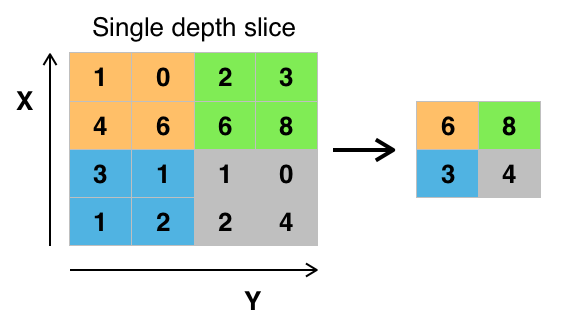
\includegraphics[scale=0.7]{charts/max_pooling.png}
			\caption{max-pooling 2 x 2}
			\label{fig:max-pooling}
		\end{figure}
		\pagebreak
		
		Công dụng của phép pooling này giúp giảm đi kích thước của tập miêu tả đặc trưng từ đó cũng làm cho số lượng tham số và tính toán giảm theo. Và do chúng ta có thể có nhiều feature map từ tầng tích chập nên phép tổng hợp cũng sẽ được áp dụng độc lập cho mỗi feature map. Nếu có 3 feature map thì sẽ có 3 phép tổng hợp trong trường hợp này là max-pooling.
		
		\begin{figure}[h!]
			\centering
			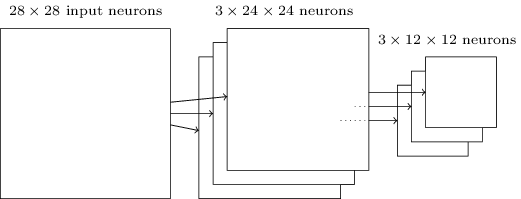
\includegraphics[scale=0.5]{charts/pooling_ex.png}
			\caption{Ví dụ tầng tổng hợp}
			\label{fig:pooling_ex}
		\end{figure}
		
	
	\subsubsection{Fully Connected Layer}
		Sau khi thông tin input đã qua các tầng tích chập và tổng hợp, các giá trị dữ liệu sẽ đi đến tầng fully connected để xuất ra kết quả. Kết quả tại tầng fully connected là một vector có kích thước bằng với số lớp(nhãn) mà bài toán cần dự đoán. Như bài toán phân loại ảnh giao thông ùn tắt và thông thoáng thì lúc này số nhãn cần dự đoán và kích thước vector tại tầng này sẽ bằng 2. Giá trị của các phần tử trong vector sẽ là giá trị xác suất của mỗi nhãn mà mạng dự đoán, [ 0.8, 0.2 ] sẽ biểu diễn 80\% ảnh này thuộc lớp 1 và 20\% ảnh thuộc lớp thứ 2. Về cơ bản, cách kết nối ở tầng này giống như cách kết nối neuron giữa các tầng với nhau ở mạng neuron ở mục trước. Khi đó, tất cả neuron ở tầng pooling sẽ kết nối với từng neuron trong tầng cuối.
	
\subsection{Kiến trúc mạng GoogLeNet)}
	
	\subsubsection{Ý tưởng}
	Đây là kiến trúc mạng tích chập với 22 tầng. GoogLeNet còn là quán quân của ILSVRC 2014 \cite{1}. Mạng googLeNet có cấu trúc mạng nằm trong mạng, có 9 tầng mà mỗi tầng là một inception module. Theo tài liệu cho biết, việc áp dụng inception module giúp làm giảm đáng kể số lượng tham số tính toán giúp giải quyết vấn đề về tài nguyên. \ref{fig:googlenet} minh họa cho cấu trúc của mạng googLeNet.
	
		
	\begin{figure}[h!]
			\centering
			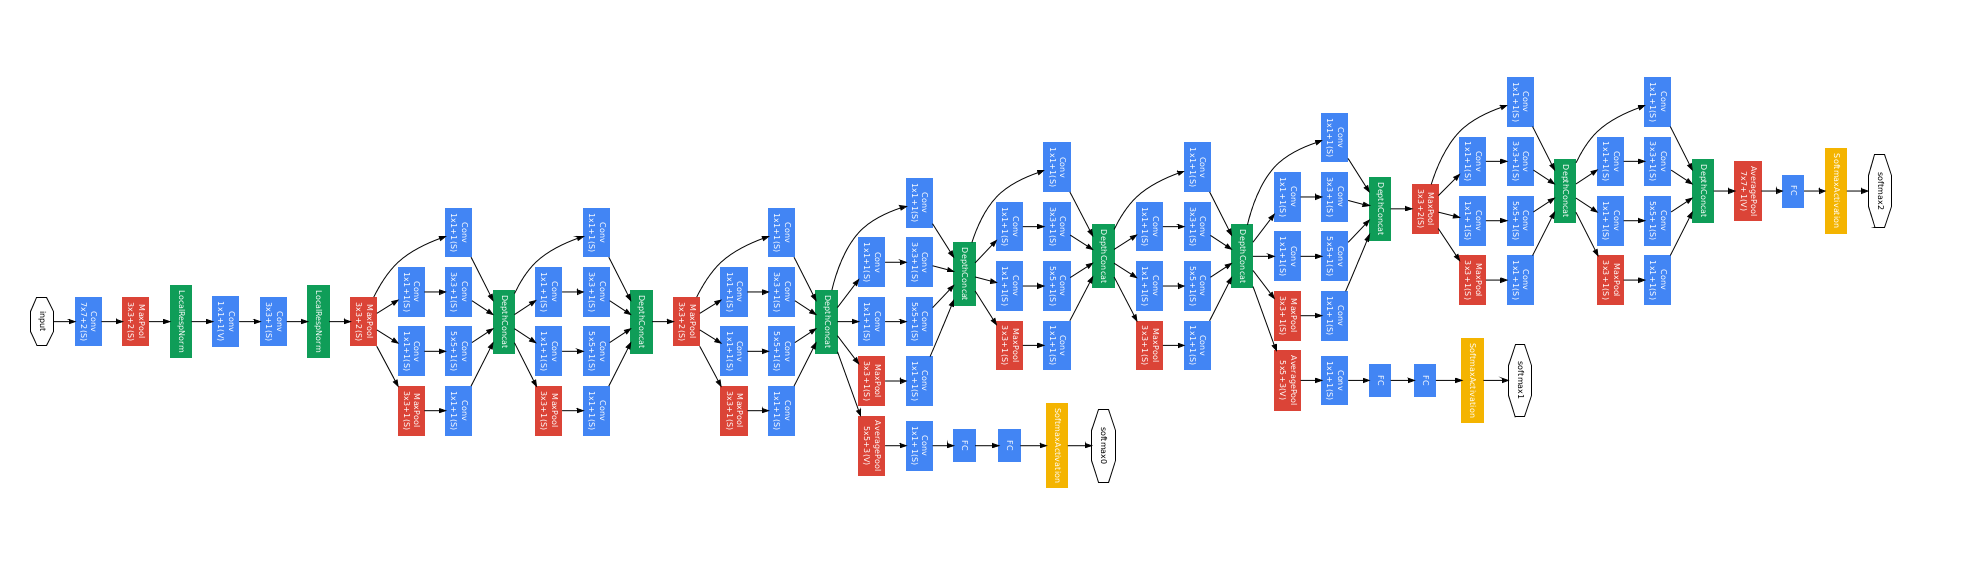
\includegraphics[scale=0.7]{charts/googlenet.png}
			\caption{GoogLeNet}
			\label{fig:googlenet}
		\end{figure}
		
	
	\subsubsection{Inception module}
	Với minh họa kiến trúc của mạng googLeNet, ta sẽ thấy các layer là một khối mạng nhỏ nằm bên trong. Đây là các inception module. Đối với các mạng tích chập thông thường, khi một tập dữ liệu bắt đầu đi vào một tầng thì sẽ chỉ có hai sự lựa chọn đó chính là tầng tích chập hoặc tầng tổng hợp, nhưng với googLeNet sẽ có tập input sẽ đi vào một lớp module tại đó sẽ các phương thức tích chập và pooling sẽ đươc tính toán một cách song song và độc lập với nhau \cite{1}.
	
	\begin{figure}[h!]
			\centering
			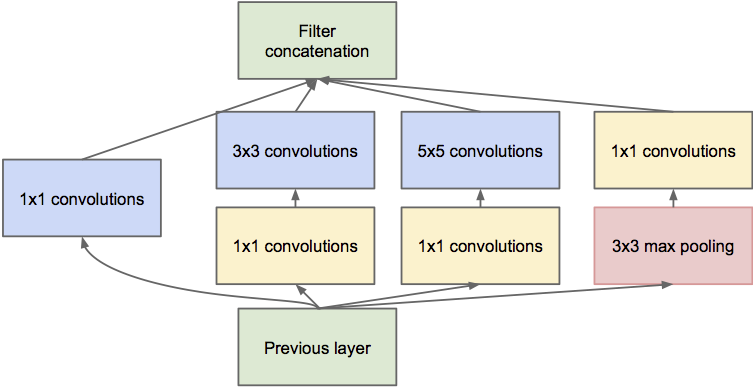
\includegraphics[scale=1.5]{charts/inception.png}
			\caption{inception module}
			\label{fig:inception}
	\end{figure}

	\begin{figure}[h!]
			\centering
			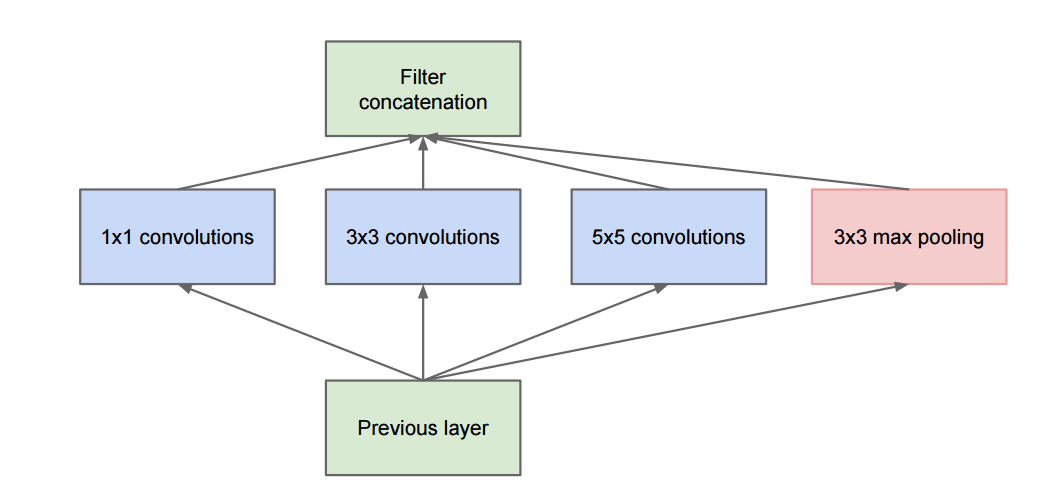
\includegraphics[scale=0.3]{charts/inception_nai.png}
			\caption{naive inception module}
			\label{fig:nai_inception}
	\end{figure}
		
	
	
	Hình \ref{fig:inception} miêu tả cấu trúc của một module trong mạng. Trong khi đó \ref{fig:nai_inception} là một ý tưởng ban đầu mà tác giả đã nghĩ tới. Ở \ref{fig:inception} chúng ta thấy trước khi thực hiện các phép tích chập với các filter 3 x 3 và 5 x 5, input đều được xử lý qua phép tích chập với filter 1 x 1. Các bộ lọc 1 x 1 có tác dụng làm giảm đi chiều của các input\cite{2}, điều này giúp cho khối lượng tham số phải tính toán ở phép toán tích chập với bộ lọc 3 x 3 và 5 x 5 sẽ được giảm đi một cách đáng kể.
		
	
	
	
	
	
\newpage\cleardoublepage
\chapter{Apache Hadoop}
\section{Tổng quan về hệ thống Apache Hadoop}
Apache Hadoop là một dự án phát triển phần mềm nhằm cung cấp một nền tảng phân tán, có thể mở rộng linh hoạt và có độ tin cậy cao.\\
Ngoài ra Hadoop còn được xem là một thư viện hay framework cho phép xử lý phân tán khối lượng lớn dữ liệu trên nhiều cụm máy tính bằng các mô hình lập trình. Framework nay được thiết kế với mục đích có khả năng mở rộng từ một máy chủ đơn lẻ lên đến rất nhiều trạm làm việc mà mỗi máy trạm có khả năng tính toán và lưu trữ cục bộ.
\section{Hadoop distributed file system - HDFS}
\subsection{Thiết kế}
HDFS là một hệ thống file nhằm lưu trữ một lượng rất rất lớn (Lớn ở đây theo nghĩa có thể là hàng trăm megabytes, gigabytes, hoặc terabytes) với cơ chế streamming data access trên những thiết bị phổ thông \footnote{các máy tính hoặc máy trạm}.
 Đây là cơ chế phân luồng dữ liệu trong HDFS với mục đích ghi một lần chạy nhiều lần. Điển hình là dữ liệu sẽ được sinh và sao chép từ nguồn và sau đó có rất nhiều tiến trình phân tích khác nhau thực thi dữ liệu trên. Mỗi hoạt động phân tích sẽ thực thi liên quan đến một phần nào đó khác nhau trên cả một tập dư liệu trên.\\
 Từ các thiết bị phổ thông ở đây là những những thiệt bị phân cứng máy tính, HDFS không yêu cầu một phần cứng đắt tiền hay độ tin cậy cao. Mà nó được thiết kế để chạy trên những cụm máy tính từ nhiều nhà cung ứng khác nhau. Vì thế mà xác suất để một node(đơn vị phần cứng) gặp lôi và thất bại là rất lớn, đặc biệt là những cụm có hàng ngàn máy trạm. Với đặc tính đó, HDFS được thiết kế sao cho không có sự gián đoạn nào được phát hiện ở người dùng khi mà việc một số lượng node gặp lỗi giữa chừng.
\subsection{Ý tưởng chủ đạo}
\newpage\cleardoublepage
\chapter{Hiện thực mô hình}

\begin{figure}[h!]
		\centering
		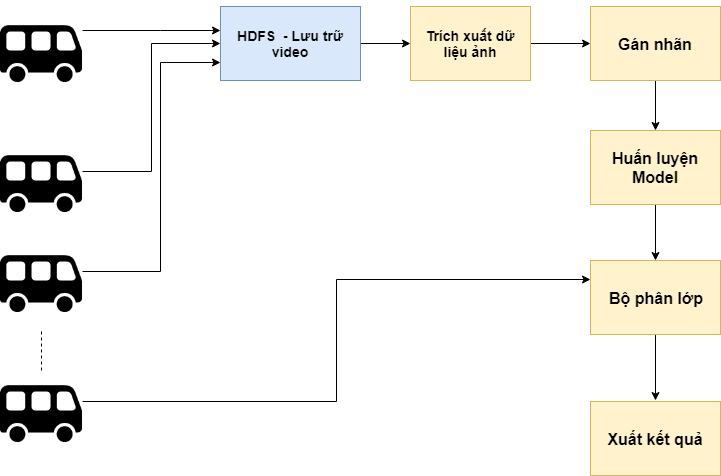
\includegraphics[scale=0.5]{charts/usecase.png}
		\caption{Mô hình phân loại ảnh giao thông kết hợp Hadoop}
		\label{fig:usecase}
	\end{figure}

\section{Tổng quan các bước}
	Hệ thống phân loại ảnh kết hợp Apache Hadoop và mô hình học sâu Deeplearning sẽ được thực hiện dựa trên sơ đồ trên. Hiện nay, các xe buýt đều được trang bị camera hanh trình và hệ thống GPS. Các video được ghi lại sẽ được lưu tại một nơi. Do số lượng của các video được gửi về liên tục và hàng ngày và giờ, nên việc sử dụng hệ thống lưu trữ HDFS của Apache Hadoop là lựa chọn hợp lý. Tiếp đến là việc truy xuất ảnh từ video và gán nhãn ảnh phục vụ cho việc huấn luyện mô hình học sâu. Đây cũng là công đoạn tốn kém chi phí nhất. Sau cùng là việc huấn luyện tập dữ liệu đã xây dựng.

\section{Các bước chuẩn bị}
\subsection{Chuẩn bị môi trường hiện thực}
	Bộ phân loại ảnh giảo hông được huấn luyện trên nền tảng hệ điều hành Linux, ngôn ngữ Python phiên bản 3.6 kết hợp với thư viện Tensorflow mã nguồn mở chuyên được sử dụng cho những mô hình học sâu.\par
	Tensorflow\cite{tf} là một thư viện học sâu mã nguồn mở được Google phát triển. Thư viện này đã thu hút được sự chú ý lớn từ cộng đồng Deep-learning. Tensorflow cho phép chạy các thuật toán machine learning trên nhiều GPU, có nhiều module được dựng sẵn giúp cho việc xây dựng và thực thi mô hình đơn giản hơn. \par
	\textbf{Các khái niệm:}
	\begin{itemize}
		\item \textbf{Tensor:} đây là cấu trúc dữ liệu được sử dụng hoàn toàn trong Tensorflow. Hay nói cách khác, tất cả dữ liệu đều biểu diễn dưới dạng tensor. Đơn giản, tensor là một mảng gồm n chiều hay list kèm theo một số thuộc tính khác.
		
		\item \textbf{Rank:} còn được gọi là số chiều của dữ liệu
		\begin{table}[h!]
			\centering
			\begin{tabular}{ | c | c | c | }
 			\hline
 			 \textbf{Rank} & \textbf{Đơn vị số} & \textbf{Ví dụ}\\
 			\hline
 			0  & Scalar  & s = 123  \\
			\hline
			1 & Vector & s = [0.8, 0.1, 0.1]	\\
			\hline
			2 & Matrix & s = [[1,2,3], [4,5,6], [7,8,9]]	\\
			\hline
			3 & 3-Tensor & s = [ [ [1], [2], [3] ], [ [4], [5], [6] ], [ [7], [8], [9] ] ]	\\
			\hline
			n & n-Tensor & n chiều dữ liệu... \\
			\hline
			
		\end{tabular}
		\caption{Các chiều dữ liệu.}
		\label{table:rank}
		\end{table}
		
		
		
		
		\item \textbf{Shape:} biểu diễn chiều của tensor. Ví dụ, \(t = [[1,2,3], [4,5,6], [7,8,9]]\) có shape là \([3, 3]\), \(t = [ [ [1], [2], [3] ], [ [4], [5], [6] ], [ [7], [8], [9] ] ]\) có shape là \([1, 3, 3]\),...
		
		\item \textbf{Type:} là các kiểu dữ liệu được sử dụng trong Tensorflow. Một vài kiểu dữ liệu cơ bản như.\\
		\begin{table}[h!]
			\centering
			\begin{tabular}{ | c | c | c | }
 			\hline
 			 \textbf{Data type} & \textbf{Python code} & \textbf{Mô tả}\\
 			\hline
 			\textit{DT-FLOAT}  & tf.float32  & 32 bits floating point.  \\
			\hline
			\textit{DT-DOUBLE} & tf.float64 & 64 bits floating point.\\
			\hline
			\textit{DT-INT16} & tf.int16	 & 16 bits signed integer.\\
			\hline
			\textit{DT-INT32} & tf.int32	 & 32 bits signed integer.	\\
			\hline
			\textit{DT-INT64} & tf.int64	 & 64 bits signed integer. \\
			\hline
			... & ... & ...\\
			\hline
			
		\end{tabular}
		\caption{Một vài kiểu dữ liệu.}
		\label{table:type}
		\end{table}
		\pagebreak
		
		
	\end{itemize}
	
	

\section{Các bước hiện thực}

	\subsection{Cài đặt Apache Hadoop}
	Trong phần hướng dẫn này chúng ta sẽ biết được cách cài đặt một cụm gồm nhiều máy Hadoop. Thông qua nhiều bước,ta sẽ biết cách cấu hình cũng như khởi tạo và kết thúc hoạt động của một cụm máy Hadoop.\par 
	\subsubsection{Cấu hình cần thiết để cài đặt một cụm 3 máy hadoop}
	Một cụm Hadoop có thể rất nhiều máy, nhưng để có được cái nhìn tổng quan và vì thời gian của đề tài nên chúng ta sẽ tiến hành cài Hadoop trên 3 máy tính. Việc bổ sung thêm máy trạm vào cụm sẽ được hướng dẫn ở nội dung cuối phần này.\par 
	\begin{itemize}
		\item \textbf{Số lượng máy tính: } 3 máy tính.
		\item \textbf{Hệ điều hành: } sử dụng hệ điều hành Ubuntu phiên bản 14.04 hoặc 16.04 hoặc cao hơn.
		\item \textbf{Phiên bản Apache Hadoop: }Gói cài đặt \href{http://hadoop.apache.org/releases.html}{Hadoop phiên bản 3.1.0}
	\end{itemize}
	\subsubsection{Cài đặt Hadoop trên máy Master(Namenode)}
	Mục này được thực hiện chỉ riêng trên máy được chọn làm Master.
		\begin{enumerate}
			\item \textbf{Các vấn đề trước khi cài đặt Hadoop:}
			\begin{itemize}
			
				\item \textbf{Thêm địa chỉ IP đầu vào vào file \textit{/etc/hosts}}				
				\begin{lstlisting}[caption=Nội dung file /etc/hosts]
	127.0.0.1	localhost
	127.0.1.1	master
	192.168.1.50	master
	192.168.1.61	slave
	192.168.1.73	slave1

				\end{lstlisting}
				Chúng ta bỏ qua 2 dòng đầu của file va chú ý tới 3 dòng tiếp theo. Bên cột trái, đó chính là lần lượt địa chỉ IP của 3 máy sẽ cài Hadoop. 192.168.1.50 là máy được chọn làm master và từ \textit{master} bên cột phải là hostname của máy đó. Tương tự 2 dòng cuối, đó là IP của 2 máy được chọn làm datanode và hostname lần lượt là \textit{slave, slave1}.\par 
				\item \textbf{Cài đặt Java:} hiện nay, Java được cài ở đây sẽ có phiên bản là Java 8. Thực hiện lần lượt các lệnh sau trên terminal để cài đặt Java 8.
				
				\begin{lstlisting}[language=python,caption=Cài đặt Java 8]
	sudo add-apt-repository ppa:webupd8team/java	
	sudo apt-get update	
	sudo apt-get install oracle-java8-installer
	
				\end{lstlisting}
				
				\item \textbf{Cấu hình SSH: } Thực hiện lần lượt các lệnh sau để cài cũng như cấu hình kết nối SSH máy master tới các máy datanodes.
				
				\begin{lstlisting}[caption=Cài đặt SSH]
	sudo apt-get install openssh-server openssh-client	
	ssh-keygen -t rsa -P ""	
				\end{lstlisting}
				Sao chép nội dung file .ssh/id\_rsa.pub của máy master đến file .ssh/authorized\_keys của máy master cũng như các máy datanodes. Sau đó kiểm tra kết nối đã thành công hay chưa bằng lệnh.\par
				\begin{lstlisting}[caption=Kết nối SSH]
	ssh slave
	ssh slave1
				\end{lstlisting}
				
			\end{itemize}
			\item \textbf{Cài đặt Hadoop}
			\begin{itemize}
				\item \textbf{Tải gói cài đặt: }Tải gói cài đặt Hadoop theo link phía dưới\\
				http://hadoop.apache.org/releases.html
				\item \textbf{Giải nén gói cài đặt: }Giải nén đến thu mục \textit{/usr/local} bằng câu lệnh
				\begin{lstlisting}
tar xzf hadoop-3.1.0.tar.gz -C /usr/local/
				\end{lstlisting}
				\item \textbf{Chỉnh sửa ~/.bashrc: }Thêm các biến môi trường cài đặt Hadoop vào file ~/.bashrc như nội dung sau.
		
				\begin{lstlisting}[language=bash]
export HADOOP_PREFIX="/usr/local/hadoop-3.1.0"
export PATH=$PATH:$HADOOP_PREFIX/bin
export PATH=$PATH:$HADOOP_PREFIX/sbin
export HADOOP_MAPRED_HOME=${HADOOP_PREFIX}
export HADOOP_COMMON_HOME=${HADOOP_PREFIX}
export HADOOP_HDFS_HOME=${HADOOP_PREFIX}
export YARN_HOME=${HADOOP_PREFIX}
				\end{lstlisting}
				Sau khi lưu nội dung chỉnh sửa, thưc thị \textit{source ~/.bashrc} để các biến hệ thống thiết lập các biến môi trường.
				\item \textbf{Cấu hình file hadoop-env.sh: }cấu hình biến \textit{JAVA\_HOME}
				\begin{lstlisting}[language=bash]
export JAVA_HOME=/usr/lib/jvm/java-8-oracle/
				\end{lstlisting}
				Thay đổi đường dẫn \textit{JAVA\_HOME} nếu cài đặt Java 8 ở một nơi khác.
				\item \textbf{Cấu hình file core-site.xml: }thêm các dòng sau
				\begin{lstlisting}[language=XML]
<configuration>
<property>
	<name>fs.defaultFS</name>
	<value>hdfs://master:9000</value>
</property>
<property>
	<name>hadoop.tmp.dir</name>
	<value>/home/'your\_user'/hdata</value>
</property>
</configuration>
				\end{lstlisting}
				\item \textbf{Cấu hình file hdfs-site.xml: }thêm các nội dung như sau
				\begin{lstlisting}[language=XML]
<configuration>
<property>
	<name>dfs.replication</name>
	<value>2</value>
</property>
</configuration>
				\end{lstlisting}
				\item \textbf{Cấu hình file mapred-site.xml: }thêm các nội dung như sau
				\begin{lstlisting}[language=XML]
<configuration>
<property>
	<name>mapreduce.framework.name</name>
	<value>yarn</value>
</property>
</configuration>
				\end{lstlisting}
				\item \textbf{Cấu hình yarn-set.xml: }thêm các nội dung như sau
				\begin{lstlisting}[language=XML]
<configuration>
<property>
	<name>yarn.nodemanager.aux-services</name>
	<value>mapreduce_shuffle</value>
</property>
<property>
	<name>yarn.resourcemanager.scheduler.address</name>
	<value>master:8030</value>
</property>
<property>
	<name>yarn.resourcemanager.address</name>
	<value>master:8040</value>
</property>
</configuration>
				\end{lstlisting}
				\item \textbf{Cấu hình file workers: }thêm hostname của 3 máy trạm mà đã đặt ở file \textit{/etc/hosts}
				\begin{lstlisting}
master
slave
slave1
				\end{lstlisting}
			\end{itemize}
			
			
			
		\end{enumerate}
		
		\subsubsection{Cài đặt Hadoop trên các datanodes}
		\begin{enumerate}
			\item \textbf{Các cấu hình chuẩn bị: }
			\begin{itemize}
				\item \textbf{Thêm địa chỉ IP vào file /etc/hosts: }thực hiện giống như đã làm ở máy master
				\item \textbf{Cài đặt Java 8}
			\end{itemize}
			\item \textbf{Cài đặt Hadoop cho tất cả máy datanodes: }thao tác này sẽ được thực hiện trên terminal của máy master.
			\begin{itemize}
				\item \textbf{sử dụng SSH để gửi file cài đặt: }thực hiện lần lượt các lệnh sau để gửi file cài đặt hadoop tới các máy datanodes
				\begin{lstlisting}
scp /usr/local/hadoop-3.1.0 slave:/usr/local/hadoop-3.1.0
scp /usr/local/hadoop-3.1.0 slave1:/usr/local/hadoop-3.1.0
				\end{lstlisting}
				Sau các lệnh này được thực thi xong thì các máy datanodes đã được cài đặt hadoop thành công
				\item \textbf{Cấu hình file ~/.bashrc: }chúng ta có thể copy nội dung từ file \textit{~/.bashrc} của master đến các máy datanodes.
			\end{itemize}
			
			\item \textbf{Khởi động cụm máy Hadoop: }chạy các lệnh sau để khởi động Hadoop
			\begin{itemize}
				\item \textit{bin/hdfs namenode -format}
				\item \textit{sbin/start-dfs.sh}			
			\end{itemize}
			\item \textbf{Kiểm tra xem Hadoop service:} lần lượt thực thi lệnh jps từ terminal của các máy master và datanode để kiểm tra, nếu kết quả như hình dưới đây thì các service hadoop đang hoạt động.
			\begin{figure}[h!]
				\centering
				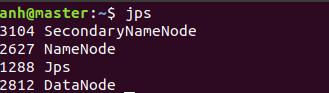
\includegraphics[scale=0.8]{charts/jps-m.png}
				\caption{Kiểm tra Hadoop service trên master}
				\label{fig:jps-m}
			\end{figure}
			\begin{figure}[h!]
				\centering
				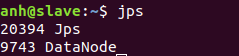
\includegraphics[scale=0.8]{charts/jps-s.png}
				\caption{Kiểm tra Hadoop service trên worker(slave)}
				\label{fig:jps-s}
			\end{figure}
			\begin{figure}[h!]
				\centering
				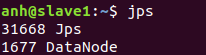
\includegraphics[scale=0.8]{charts/jps-s1.png}
				\caption{Kiểm tra Hadoop service trên worker(slave1}
				\label{fig:jps-s1}
			\end{figure}
			
			
		\end{enumerate}
		
	\subsubsection{Thêm một datanodes vào một cụm Hadoop đang hoạt động}
	Trong quá trình sử dụng, việc muốn mở rộng cụm máy Hadoop là điều có thể xảy ra. Chúng ta có thể dễ dàng thêm một datanodes và một cụm máy Hadoop đang hoạt động theo các bước sau.
	\begin{enumerate}
		\item \textbf{Cài đặt Java 8: }đảm bảo rằng máy được thêm vào cụm phải được cài đặt Java 8 như đã trình bày ở phía trên.
		\item \textbf{Thêm địa chỉ IP vào /etc/hosts: }thêm địa chỉ IP của máy datanode mới vào file /etc/hosts của máy master và các máy datanodes đã có cũng như datanode mới.
		\item \textbf{Cấu hình SSH: }copy nội dung file ~/.ssh/id\_rsa.pub vào máy datanodes mới giống như đã làm với các máy datanode đã trước.
		\item \textbf{Cài đặt Hadoop: }chúng ta cũng sử dụng SSH để gửi thư mục cài Hadoop từ máy master sang máy datanode mới như đã thực hiện.
		\item \textbf{Cấu hình file workers: }thêm hostname của máy datanode mới vào file workers trên máy master.
		\item \textbf{Khởi động datanode: }thực hiện file \textit{start-dfs.sh} trong thư mục sbin trên máy master để tiến hiện khởi động datanode mới vào cụm máy.
	\end{enumerate}
		
	\subsubsection{Lưu trữ dữ liệu ảnh trên HDFS}
	Để đưa dữ liệu lên HDFS, ta sử dụng câu lệnh sau.
	\begin{lstlisting}
hdfs dfs -put ~/Document/traffic/ hdfs://master:9000/
	\end{lstlisting}
	Với \textit{~/Document/traffic} là đương dẫn đến thư mục lưu dữ liệu ảnh, và \textit{hdfs://master:9000/} là đường dẫn đến vị trí lưu của HDFS. Để xem kết quả put ta thực hiện lệnh sau để liệt kê các thư mục dữ liệu đã được lưu trên HDFS.
	\begin{figure}[h!]
				\centering
				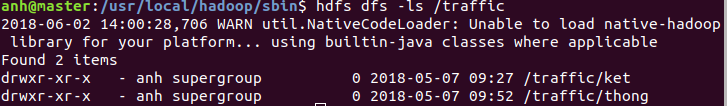
\includegraphics[scale=0.6]{charts/dfs-ls.png}
				\caption{Liệt kê thư mục dữ liệu trên HDFS}
				\label{fig:dfs-ls}
	\end{figure}
	
	\subsection{Cài đặt HIVE}
	Để cài đặt HIVE và lưu trữ dữ liệu GPS, ta thực hiện các bước sau đây.
	\subsubsection{Tải gói cài đặt HIVE}
	Tải gói cài đặt HIVE ở với đường dẫn sau \textit{http://mirror.downloadvn.com/apache/hive/}, ta sẽ sử dụng phiên bản 2.2.0.
	\subsubsection{Cài đặt HIVE}
	\begin{enumerate}
		\item \textbf{Giải nén: }giải nén gói cài đặt và copy thư mục có được vào vị trí thư mục muốn cài chẳng hạn như \textit{/usr/local/hive}.
		\item \textbf{Cấu hình biến môi trường: }thêm vào file \textit{~/.bashrc} nội dung như sau
		\begin{lstlisting}[language=bash]
export HIVE_HOME=/usr/local/hive
export PATH=$PATH:$HIVE_HOME/bin
export CLASSPATH=$CLASSPATH:/usr/local/Hadoop/lib/*:.
export CLASSPATH=$CLASSPATH:/usr/local/hive/lib/*:.
	\end{lstlisting}
	Thực hiện lệnh \textit{source ~/.bashrc} để thực thi cấu hình.
	\end{enumerate}
	
	\subsubsection{Tải và cài đặt Apache Derby}
	Làm theo các lệnh hướng dẫn để tải à cài đặt Apache Derby
	\begin{enumerate}
		\item \textbf{Tải Apache Derby: } vào và tải ở địa chỉ sau \textit{http://archive.apache.org/dist/db/derby/} với phiên bản 10.14.2.0
		\item \textbf{Giải nén: } giải nén vào thư mục \textit{/usr/local/derby}
		\item \textbf{Cấu hình biến môi trương cho Derby:} Thêm nội dung file \textit{~/.bashrc} như sau.
		\begin{lstlisting}[language=bash]
export DERBY_HOME=/usr/local/derby
export PATH=$PATH:$DERBY_HOME/bin
		\end{lstlisting}
	\end{enumerate}
		
	\subsubsection{dữ liệu GPS }
	Dữ liệu GPS là tập dữ liệu lưu vị trí GPS của một xe buýt trong một thời điểm nhất định. Dữ liệu này được lưu bằng bảng trong HIVE. Cấu trúc của bảng dữ liệu bao kinh độ, vĩ độ, thơi điểm theo định dạng DD/MM/YYYY hh:mm:ss.
	
	

	\subsection{Xử lý dữ liệu}
	
	Để xây dựng mô hình phân loại hình ảnh, chúng ta cần phải có một tập huấn luyện đủ tốt. Ở đây, các hình ảnh được trích xuất từ camera hành trình từ các tuyến xe buýt. \par
	Cấu trúc tổ chức tập dữ liệu gồm 2 thư mục chính:
	\begin{itemize}
		\item Thư mục \textbf{ket}: chứa các hình ảnh được cho là giao thông trong tình trạng ùn tắt. Bao gồm khoảng 7500 hình ảnh định dạng JPG.
		\item Thư mục \textbf{thong}: chứa các hình ảnh được cho là giao thông trong tình trạng thông tháng. Bao gồm 7700 hình ảnh định dạng JPG.
	\end{itemize}
	
		Các hình ảnh được trình bày và lưu trữ vào các thư mục có chứa các tên mô tả cho đặt tính của những hình ảnh đó. Với bộ dữ liệu trên, chương trình tạo một kiểu dữ liệu dictionary với khóa chính là giá trị biểu diễn cho tên thư mục và cũng là tên class cần phân loại, value chính là đường dẫn các file ảnh tương ứng.\par
		 Để sử dụng được trong mô hình mạng, các hình ảnh sẽ được mã hóa sang một định dạng mới nhờ các phương thức hỗ trợ có sẵn trong thư viện Tensorflow. Sau khi được mã hóa, kết quả chính là các tensor có thông số shape như sau [299, 299, 3], với hai vị trí đầu tiên chính là kích thước của hình ảnh cũng như của tensor, giá trị 3 biểu diễn cho độ sâu (ảnh màu).\par
	 	Sau cùng, bộ dữ liệu đã được mã hóa được chia thành 3 tập con sử dụng với 3 mục đích khác nhau: tập huấn luyện(Training set), tập validation để tránh vấn đề overrfit trong quá trình huấn luyện và tập kiểm thử dùng để kiểm tra độ chính xác của mô hình sau khi huấn luyện hoàn tất.	Riêng tập huấn luyện sẽ được dùng để tạo ra các bottlenecks
	
	\subsection{Tạo các bottlenecks}
	
	Bottlenecks\cite{bottlenecks} là một từ được dùng để chỉ tầng (layer) nằm ngay trước fully-connected layer. Với kiến trúc mạng googLeNet, tầng này đã được huấn luyện tập dữ liệu trước đó nên có được kết quả đủ tốt để phân biệt được đặc tính của mỗi lớp(class) yêu cầu. Có nghĩa ở bước này chúng ta sẽ tạo ra một bản tóm tắt các giá trị trọng số đủ tốt cho mỗi ảnh input. Tầng cuối cùng của kiến trúc mạng sẽ sử dụng các giá trị bottlenecks này để huấn luyện và điều chỉnh để phân loại các lớp mới. Điều này nhờ vào việc mạng đã được huấn luyện bởi tập dữ liệu gồm 1000 lớp khác nhau của ImageNet giúp cho việc phát hiện các mẫu đặc tính trở nên dễ dàng hơn.
	
	\subsection{Huấn luyện}
		
	Sau khi hoàn tất tạo các giá trị bottleneck, việc thực hiện thực hiện cấu hình mạng và huấn luyện bắt đầu. Tổng số bước huấn luyện sẽ được cài đặt mặc định là 4000 bước, tuy nhiên có thể thay đổi lại tùy theo tình huống. Mỗi bước huấn luyện sẽ chọn ra 100 dữ liệu ngẫu nhiên \footnote{Tập dữ liệu lúc này là những bottlenecks} để đưa vào tầng cuối cùng \footnote{Tầng fully-connected với softmax là activation function} để dự đoán lớp, lớp dự đoán sẽ được so sánh với các lớp thực tế để mạng điều chỉnh và cập nhật các giá trị trọng số thông qua cơ chế lan truyền ngược như đã trình bày ở chương trước. Do phép toán được thực hiện trên tập huấn luyện nên sẽ  gây ra vấn đề overfit, vì thế mà tập validation sẽ được sử dụng để đo lại giá trị sai lệch và độ chính xác. Nếu độ chính xác tại tập huấn luyện cao nhưng tại tập validation không thay đổi hoặc thấp thì chứng tỏ mô hình mạng gặp phải vấn đề overfit và việc huấn luyện tiếp tục không còn có ích.
	
	\subsection{Chạy Huấn luyện bằng cách kết hợp tensorflow với hệ thống HDFS}
	\subsubsection{Chuẩn bị}
	Ở các nội dung trên, chúng ta đã thực hiện việc cài đặt Apache Hadoop cũng như các biến môi trường cần thiết, trong đó có hai biến môi trường cần thiết để chạy thực thi mô hình trên là \textbf{JAVA\_HOME} và vị trí cài đặt Hadoop\textbf{HADOOP\_HDFS\_HOME}. Bây giờ chúng ta sẽ cần thêm một biến môi trường cho hệ thống nữa.
	\begin{itemize}
		\item \textbf{LD\_LIBRARY\_PATH: }để thêm biến này, chúng ta cần thêm vào file \textit{~/.bashrc} nội dung như sau.	
	\begin{figure}[h!]
			\centering
			
\includegraphics[scale=0.8]{charts/ldlib.png}
			\caption{Nội dung thư viện LD\_LIBRARY\_PATH}
	\end{figure}
		
	\end{itemize}
	\subsubsection{Chạy mô hình huấn luyện.}
	Chúng ta thực hiện câu lệnh sau đây để tiến hành chạy mô hình huấn luyện kết nối với tập dữ liệu ở HDFS.
	\begin{figure}[h!]
			\centering
			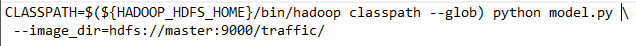
\includegraphics[scale=0.8]{charts/run.png}
			\caption{Câu lệnh thực thi huấn luyện mô hình}
	\end{figure}

\newpage\cleardoublepage
\chapter{Kết quả huấn luyện và đánh giá}
\section{Kết quả huấn luyện}
Với các thông số mạng đã cấu hình ở chương trước, việc huấn luyện mạng mang lạikết quả tương đối tốt với giá trị \(cross_entropy = 0.29\) và độ chính xác ở tập kiểm thử là 88.7\%. Không những thế việc áp dụng kỹ thuật transfer learning giúp tiết kiệm thời gian huấn luyện gấp nhiều lần. Cụ thể, việc xây dựng mô hình thủ công và huấn luyện lại từ đầu đối với máy tính không hỗ trợ card GPU sẽ mất thời gian là 8 tiếng nhưng đối với việc áp dụng mô hình inception model với kỹ thuật transfer learning thì chỉ mất từ 45 đến 60 phút để hoàn thành.\par

	\begin{figure}[h!]
		\centering
		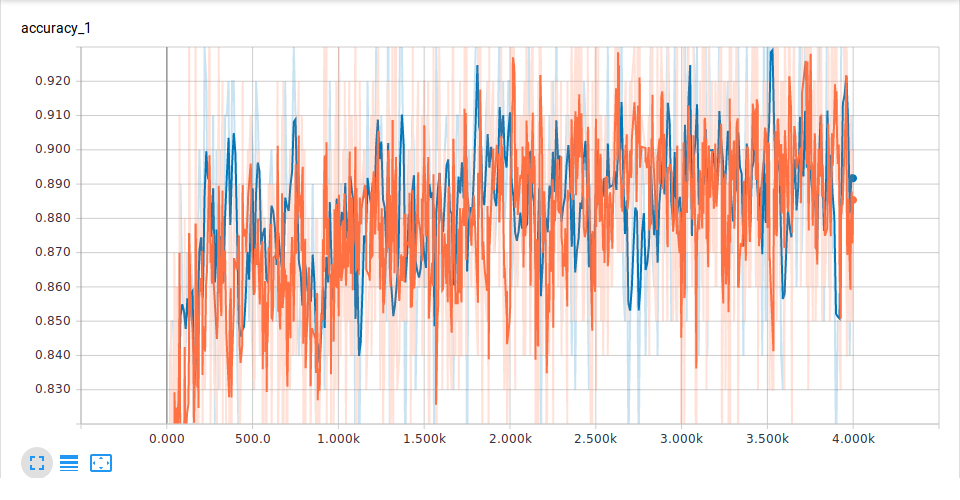
\includegraphics[scale=0.5]{charts/accuracy.png}
		\caption{Đồ thị biểu diễn độ chính xác (accuracy)}
		\label{fig:accuracy}
	\end{figure}

Đồ thị \ref{fig:accuracy} biểu diễn chi tiết độ chính xác trong quá trình huấn luyện với đường màu cam biểu diễn cho quá trình huấn luyện và đường màu xanh lam biểu diễn cho kiểm tra trên tập Validation. Tương tự với \ref{fig:cross_entropy}.

	\begin{figure}[h!]
		\centering
		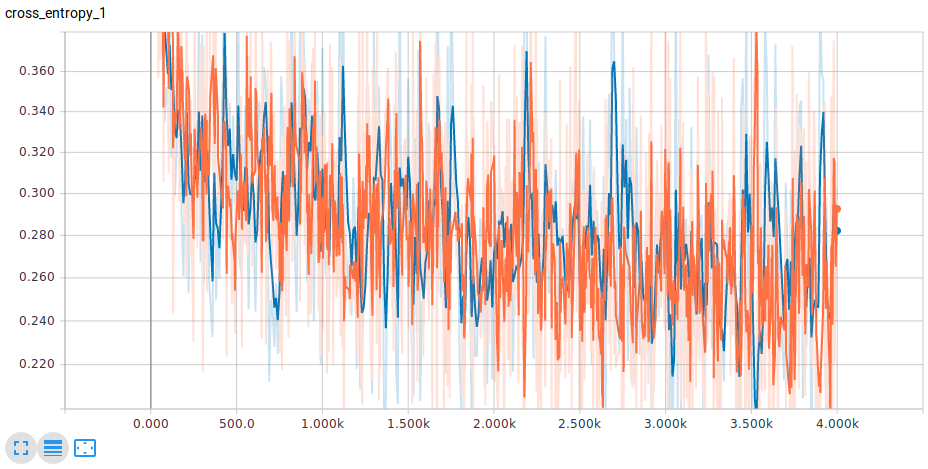
\includegraphics[scale=0.5]{charts/cross-entropy.png}
		\caption{Đồ thị biểu diễn độ sai số (cross entropy)}
		\label{fig:cross_entropy}
	\end{figure}

\section{Sử dụng mô hình phân loại ảnh mới}
	Sử dụng mô hình để phân loại một số hình ảnh khác chưa được phân loại. Hình \ref{fig:test1} có thể nhận biết bằng mắt thường là hình ảnh của những con đường đang trong tình trạng ùn tắt. Khi đưa ảnh vào mô hình, ta thu được kết quả phân loại với hai giá trị \textit{ket} và \textit{thong} lần lươt là 0.9910778 và 0.0089. Các con số này mang ý nghĩa bộ phân lớp cho rằng tấm ảnh trên có  khoảng 99\% là thuộc về lớp kẹt xe và xấp xỉ 1\% là thuộc về lớp thông thoáng.\par 
	\pagebreak	
	\begin{figure}[h!]
		\centering
		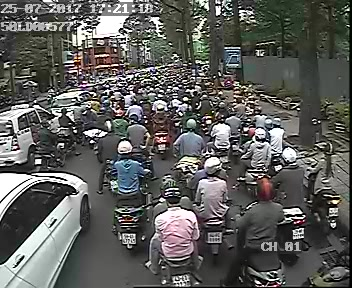
\includegraphics[scale=1]{charts/test-ket.jpg}
		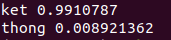
\includegraphics[scale=0.5]{charts/test-ket-res.png}
		\caption{Ảnh kiểm thử 1 - kết quả}
		\label{fig:test1}
	\end{figure}
	
	Tương tự đối với hình \ref{fig:test2}, cũng là một hình ảnh thể hiện tình trạng giao thông đang bị ùn ứ, khó khăn trong việc di chuyển. Mô hình đã đưa ra kết quả phân loại với hai giá trị \textit{ket} và \textit{thong} lần lượt là 0.9616194 và 0.038380623. Tức là 96 \% thuộc về lớp kẹt xe, 3.8\% là thuộc về lớp thông thoáng
	\begin{figure}[h!]
		\centering
		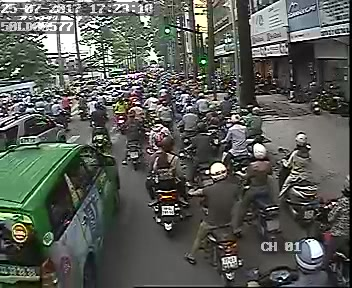
\includegraphics[scale=1]{charts/test-ket1.jpg}
		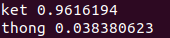
\includegraphics[scale=0.5]{charts/test-ket1-res.png}
		\caption{Ảnh kiểm thử 2 - kết quả}
		\label{fig:test2}
	\end{figure}
	
	\pagebreak
	Đối với hai hình ảnh tiếp theo được phân biệt vào loại đường thông thoáng một cách dễ dàng. Mô hình dự đoán xác suất hai hình ảnh dưới đây thuộc lớp thông thoáng lần lượt là. \par 
	
	
	Ở hình \ref{fig:test3}, khi nhìn vào camera ta có thể nhận biết được vào thời điểm này, các phương tiện trên đường rất ít, di chuyển rất dễ dàng, không xảy ra tình trạng kẹt xe hay ùn tắt nào. Mô hình cũng đã đưa ra kết quả với hai giá trị \textit{ket} và \textit{thong} lần lượt là 0.005655429 và 0.9943446. Tức là 99.4 \% thuộc về lớp thông thoáng, xấp xỉ 0.6 \% thuộc về lớp kẹt xe. \par
	\begin{figure}[h!]
		\centering
		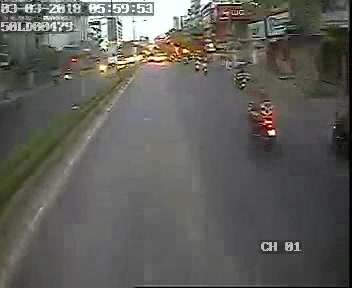
\includegraphics[scale=1]{charts/image0125.jpg}
		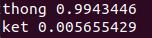
\includegraphics[scale=0.5]{charts/most-last-res.png}
		\caption{Ảnh kiểm thử 3 - kết quả}
		\label{fig:test3}
	\end{figure}
	
	Tương tự với hình \ref{fig:test4}, ta nhận thấy trong hình ảnh này, các phương tiện đang cách xe buýt một khoảng tương đối xa, mặt đường ở giữa khá thông thoáng để di chuyển. Từ đó, mô hình đã đưa ra kết quả với hai giá trị \textit{ket} và \textit{thong} lần lượt là 0.10274496 và 0.89725506. Tức là 89.7 \% thuộc về lớp thông thoáng, và xấp xỉ 10.3 \% thuộc về lớp kẹt xe. \par
	\begin{figure}[h!]
		\centering
		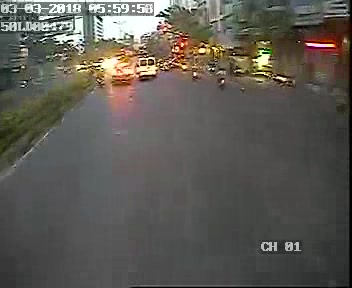
\includegraphics[scale=1]{charts/image0126.jpg}
		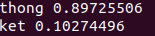
\includegraphics[scale=0.5]{charts/last-res.png}
		\caption{Ảnh kiểm thử 4 - kết quả}
		\label{fig:test4}
	\end{figure}
	\pagebreak
	Như vậy, kết quả kiểm thử đối với một số hình ảnh chưa được phân loại của mô hình đã huấn luyện cho kết quả khá chính xác. Tuy nhiên, đối với vấn đề  phân loại giao thông thì không chỉ có hai trường hợp ùn tắt hay thông thoáng mà còn tồn tại nhiều trường hợp hơn. Như tình huống đông xe nhưng di chuyển chậm, trên thực tế đây là tình huống không phải ùn tắt nhưng ảnh chụp gần giống với ảnh ùn tắt. Cần chú ý vấn đề này khi lựa chọn, phân loại ảnh huấn luyện, hoặc để giải quyết tốt hơn cần phải tăng số lượng lớp(nhãn) cần phân loại lên thành 3 hay lớn hơn thay vì 2 như ban đầu.
	
	
	\newpage\cleardoublepage
\chapter{Kết luận}

\section{Các kết quả }
Luận văn này giúp nghiên cứu, tìm hiểu về mạng học sâu cũng như việc phân loại ảnh giao thông. Các kết quả đã đạt được đáp ứng được các mục tiêu đã đặt ra.
	\begin{itemize}
		\item Xây dựng được mô hình HDFS sử dụng Apache Hadoop có thể lưu trữ dữ liệu video tập dư liệu ảnh
		\item Xây dựng được bộ dữ liệu phục vụ cho việc huấn luyện mô hình phân biệt 2 loại ảnh giao thông. Số lượng anh thu thập được trung bình mỗi lớp khoảng 1000 cho đến 2000 ảnh.
		\item Huấn luyện thành công mô hinh học sâu GoogleNet sử dụng tập dữ liệu được lưu trữ tư hệ thống HDFS.
		\item Xác định được vị trí và cho kết quả tình hình giao thông.	
	\end{itemize}
\section{Hướng phát triển}
Sau khi đạt được kết quả huấn luyện khá tốt, hướng phát triển của đề tài trong tương lai như sau:
\begin{enumerate}
	\item Tiếp tục xem xét việc xác định các lớp ảnh giảo thông trong tương lai giúp phát hiện nhiều loại hình như ùn tắt, thông thoáng, đông xe di chuyển chậm,.v.v. giúp cụ thể hóa tình trạng giao thông.
	\item Xây dựng trang web giúp nhận biết kẹt xe.
	\item Có thể sử dụng nền tảng đã xây dựng để áp dụng cho nhiều bài toán phân loại ảnh khác.
\end{enumerate}
	

Hệ thống tiềm năng trên có thể giúp dân cư sinh sống ở các khu đô thị cũng như ban quản lý nắm bắt tình hình giao thông để phân luồng di chuyển và khắc phục một cách nhanh nhất.\newpage\cleardoublepage
%\addbibresource{references.bib}
\nocite{*}
\bibliography{references}\newpage\cleardoublepage
\bibliographystyle{plain}

\end{document}
